\documentclass[border=2pt]{standalone}
\usepackage{pgfplots}
\usepackage{pgfplotstable}
\pgfplotsset{compat=1.18}
\usepackage{xcolor}
\definecolor{amber}{HTML}{E69F00}
\definecolor{teal}{HTML}{009E73}
\definecolor{blue}{HTML}{0072B2}
\definecolor{mauve}{HTML}{CC79A7}
\definecolor{grey}{HTML}{999999}
\definecolor{vermilion}{HTML}{D55E00}
\usepackage{times}

\begin{document}

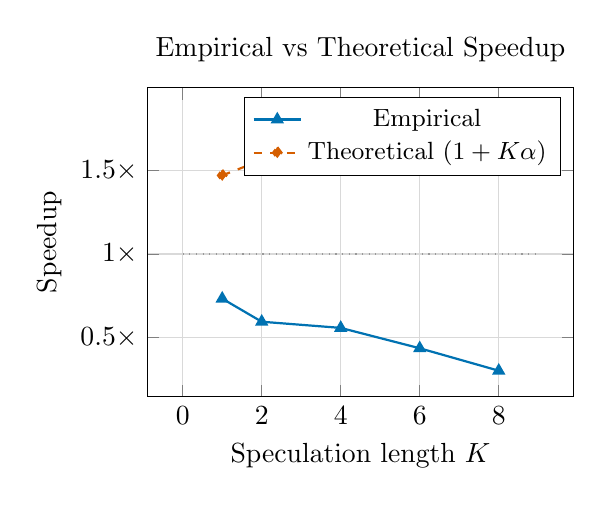
\begin{tikzpicture}
\begin{axis}[
  width=7cm, height=5.5cm,
  xlabel={Speculation length $K$},
  ylabel={Speedup},
  title={Empirical vs Theoretical Speedup},
  legend pos=north east,
  legend style={font=\small},
  grid=major, grid style={gray!30},
  yticklabel={\pgfmathprintnumber[fixed,precision=2]{\tick}$\times$},
]
\addplot[color=blue, mark=triangle*, thick] coordinates {(1,0.7323) (2,0.5939) (4,0.5569) (6,0.4348) (8,0.3004)};
\addlegendentry{Empirical}
\addplot[color=vermilion, mark=diamond*, dashed, thick] coordinates {(1,1.4706) (2,1.5625) (4,1.7611) (6,1.8000) (8,1.8411)};
\addlegendentry{Theoretical ($1+K\alpha$)}
\addplot[grey, dotted] coordinates {(0,1) (9,1)};
\end{axis}
\end{tikzpicture}
\hfill
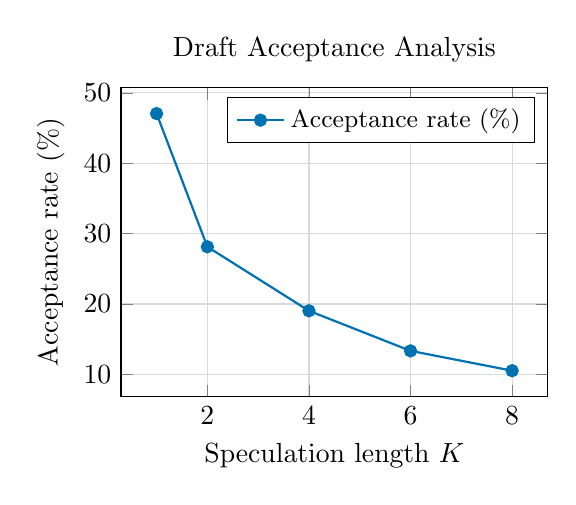
\begin{tikzpicture}
\begin{axis}[
  width=7cm, height=5.5cm,
  xlabel={Speculation length $K$},
  ylabel={Acceptance rate (\%)},
  title={Draft Acceptance Analysis},
  legend pos=north east,
  legend style={font=\small},
  grid=major, grid style={gray!30},
]
\addplot[color=blue, mark=*, thick] coordinates {(1,47.0588) (2,28.1250) (4,19.0265) (6,13.3333) (8,10.5140)};
\addlegendentry{Acceptance rate (\%)}
\end{axis}
\end{tikzpicture}
\end{document}
